\sectionname{Times Roman}

Although Times Roman does not have an ``official'' set of \MF\ parameters, we
can use the set prepared by Alan Hoenig as a reference for comparing our
measured parameters~\cite{mathkit}. There is no sense of an ``incorrect''
measurement because of this; Hoenig may just as well have erred in measurement.

\begin{figure*}
\begin{center}
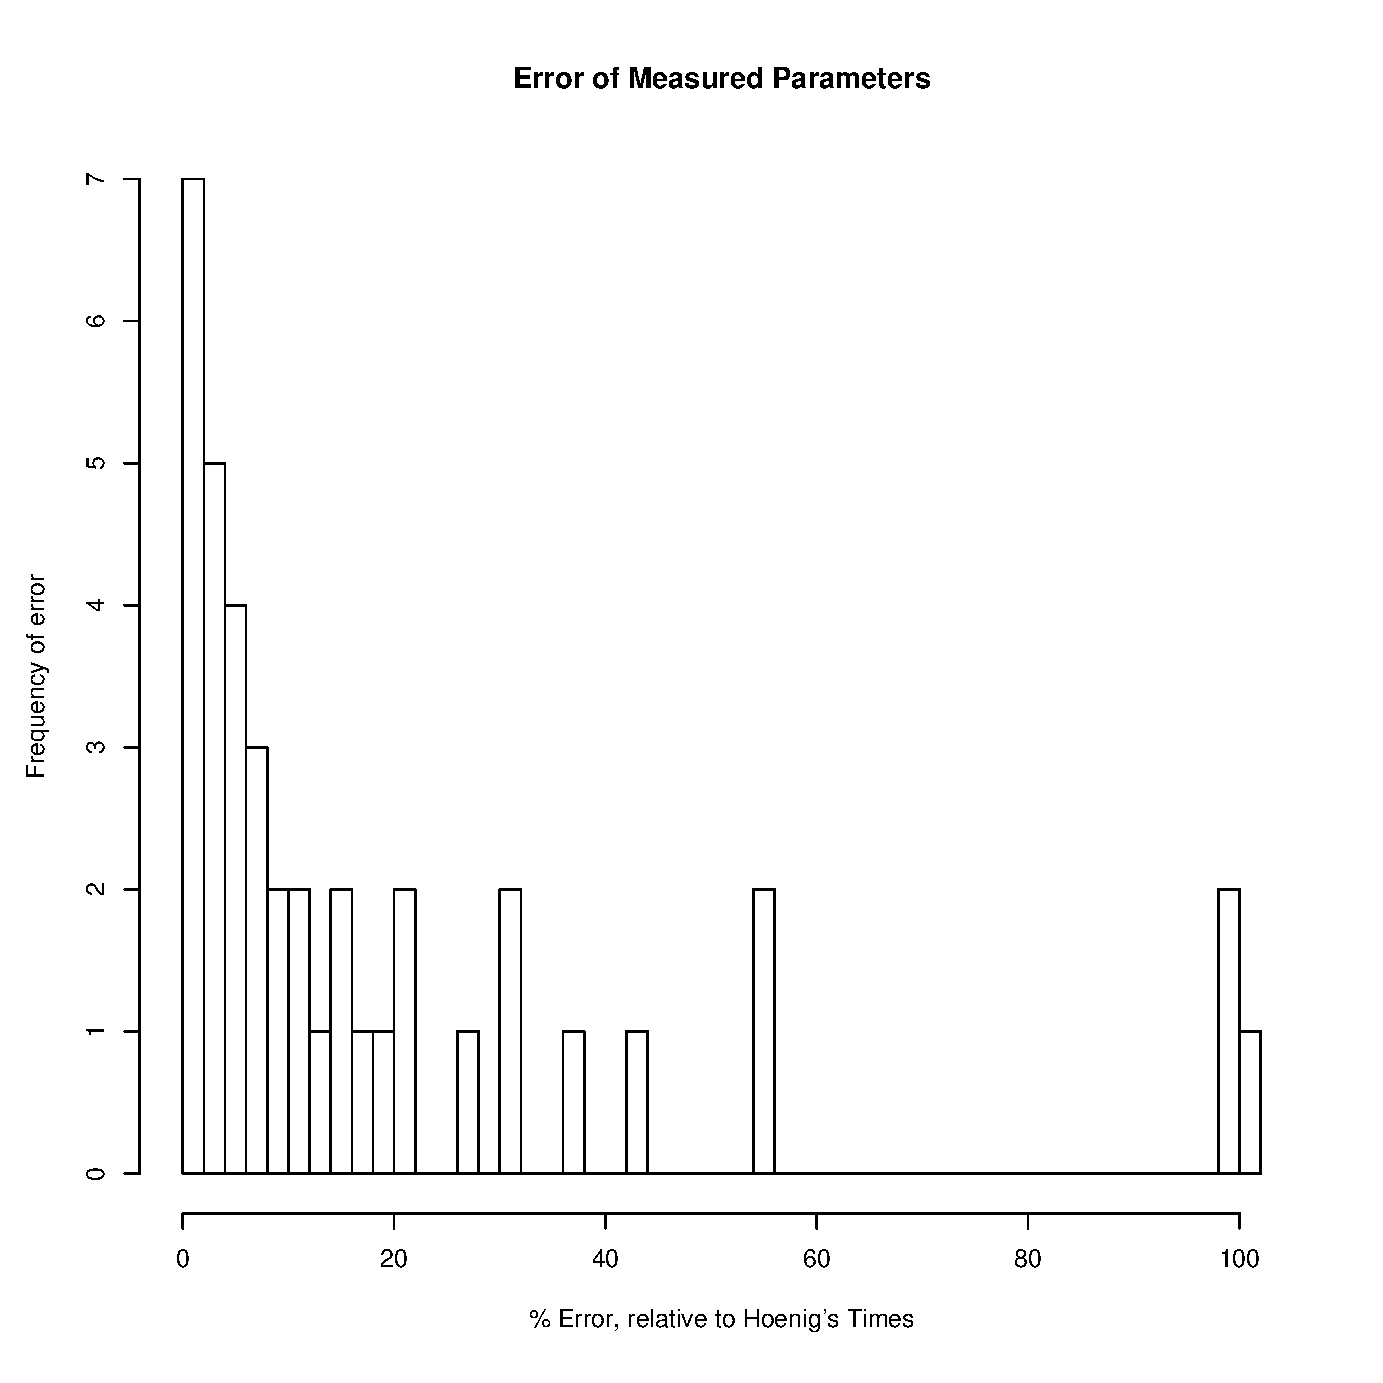
\includegraphics[width=6in]{params/times}
\end{center}
\caption{Percent error of measured parameters relative to Alan Hoenig's
parameter set, as provided in MathKit.}
\label{f:times}
\end{figure*}

As Figure~\ref{f:times} shows, the measurements for Times are substantially
different from those provided by Hoenig. In fact, on the \emph{cap\_serif\_fit}
parameter there seems to be the greatest disagreement: Hoenig's parameters
increase the whitespace around the relevant uppercase Greek characters, while
MathGen removes space (i.e., the parameter is large and positive in MathKit but
negative in MathGen).

It is difficult to resolve some of these disparities. For example, Hoenig's
values for the \emph{o} and \emph{apex\_o} parameters are both substantially
larger than MathGen's computed values.\footnote{These parameters specify the
amount by which curved letters and angled letters (e.g., o and v) should
``overshoot'' their intended heights and depths.} However, careful inspection of
the font samples and actual hand-measurement of those parameters reveal that, if
anything, they should be \emph{smaller} than those reported by MathGen. The
author's hypothesis is that Hoenig's measurements were taken on a slightly
different version of Times Roman.
